\chapter{Background}
\citationChap{
    Long ago, the world was nothing more than an endless sea cloaked in a boundless sky, reaching as far as could possibly be imagined{\ldots}
    }{Shulk (\textit{Xenoblade Chronicles})}
\minitoc
\newpage

\chapabstract{
    In this chapter, we provide some background information related to Automatic Story Generation and Evaluation ({\asg} and {\ase}). In \autoref{sec:preneural_asg}, we cover older methods for {\asg}: namely, structural and planning-based models. In \autoref{sec:language_models}, we present language models, focusing on neural-based language models, from recurrent neural networks to large language models. Finally, in \autoref{sec:eval_and_meta}, we present different aspects related to the question of evaluation in NLP.
}

\section{Pre-neural Automatic Story Generation}
\label{sec:preneural_asg}

In this section, we provide a brief history of previous work on automatic story generation which did not rely on neural networks; more detailed accounts can be found in \citet{kybartas2016survey, alhussain2021automatic}. We re-use the classification of \citet{alhussain2021automatic}, who identify three categories: structural models, planning-based models, and machine learning (\ml) models. 

\subsection{Structural Models}
\label{sub:structural_models}

A \emph{story} can be defined as ``a description of real or imaginary actors and events generated to achieve one or more goals, such as entertainment or education'' \citep{alhussain2021automatic}. In early research, a story was commonly viewed as a \emph{script}, \ie, a structure that describes a sequence of events that is coherent within a given context \citep{schank2013scripts}. Such sequences, also called \emph{schemas}, could then be used as building blocks for automatic story generation: after building a library of annotated stories, and given a schema divided into several slots, one can generate a story by retrieving matching slots from the library, as shown on \autoref{fig:structural_story_generation}.

\begin{figure}
    \centering
    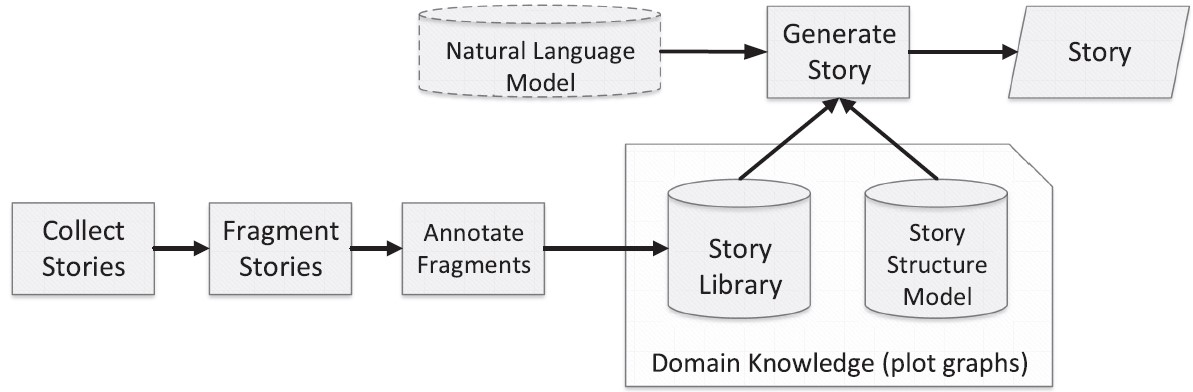
\includegraphics[width=\columnwidth]{pictures/structural_models.jpg}
    \caption{Structural story generation. Source: \citet{alhussain2021automatic}.}
    \label{fig:structural_story_generation}
\end{figure}

One of the oldest structural models is found in \citet{propp1968morphology}. They analyzed around 600 Russian folktales and distilled from them a set of 31 character actions called \emph{functions} (\eg\ departure, struggle, rescue). Their work was used in Joseph Grimes' pioneer system \citep{ryan2017grimes}, which selected random functions from \citet{propp1968morphology} and ordered them according to the model's rules.

\begin{table}
    \centering
    \begin{tabular}{p{0.8\columnwidth}}
        \toprule
        \texttt{A lion has been in trouble for a long time. A dog steals something that belongs to the lion. The hero, lion, kills the villain, dog, without a fight. The hero, lion, thus is able to get his possession back.}\\
        \bottomrule
    \end{tabular}
    \caption{The only surviving output from Joseph Grimes' system \citep{ryan2017grimes}.}
    \label{tab:grimes}
\end{table}

Scripts and schemas have been used in order to build \textbf{story graphs}. \citet{maranda1985semiography} constructed a graph based on the model from \citet{propp1968morphology} for the generation of folktales. The graph consists of nodes containing Propp's functions and of an annotated knowledge base that is searched for finding a good candidate for the next node. When a candidate is found, it is appended to the story, and this process is repeated until it reaches an end node.

Other works on narratives relied on theoretical structures called \textbf{story grammars}, which typically attempted to formalize how a sample of discourse is perceived as a coherent story, as opposed to another arrangement of the same sentences \citep{brewer1980event}. While multiple story grammars have been introduced in the literature, they all postulate the necessary components of a story and the rules that describe their relations with one another.

\citet{lakoff1972structural} is the first to have used a grammar for story generation: they adapted \citet{propp1968morphology} into a story grammar, viewing stories as words and Propp's functions as letters. \citet{grasbon2001morphological} also relied on Propp's morphology but they did not completely automate plot generation, opting instead for guiding the author along a certain story path. \citet{champagnat2010storytelling} used Campbell's Hero's Journey to create a generalized plot grammar capable of producing a high-level plot structure, also leaving the actual writing of the story to a human author. \citet{colby1973partial} developed a grammar focused on aboriginal folktales. It expanded the notion of events from Propp's model, which allowed for more unique and varied plot structures. Other grammars were proposed by \citet{rumelhart1975notes}, \citet{mandler1977remembrance}, and \citet{thorndyke1977cognitive}.

\textsc{Gester} \citep{pemberton1989modular} is one of the earliest full-fledged grammar-based plot generators. Its grammar was derived from Old French epic narratives, describing both events with causes and effects but also the relations between characters. \citet{bringsjord1999artificial} proposed \textsc{Brutus}, which relied on plot grammars for the construction of betrayal narratives. Its stories could display high complexity but were specifically geared towards plots involving events of betrayal. \citet{machado2001real} developed \textsc{Teatrix}, an interactive narrative system which created folktale templates based on Propp's functions. Author and interactor share the responsibility of the plot structure, assisted by the automatic selection of the next template and the automatic simulation of character actions. \citet{spierling2002setting} introduced \textsc{Geist}, which also creates templates for interactive stories using Propp's grammar. The stories are anchored in real world locations through augmented reality. \textsc{Squege} \citep{onuczko2008stop} uses rewrite rules to progressively build more complex structures and selecting characters to fill plot roles in a manually authored space. \citet{kybartas2013analysis} combine grammar and graph-rewriting rules in their \textsc{ReGEN} model, while also accounting for the relationships between characters.

Structural models for story generation had the advantage of being straightforward and easy to implement, but they focused primarily on the correctness of the generated story's syntax, leaving aside its semantic aspect. \citet{black1979evaluation} argued that story grammars had major deficiencies which led them to conclude that they were not a promising approach to investigating story understanding. They suggested to explore more content-oriented approaches, \eg\ planning knowledge.

\subsection{Planning-Based Models}
\label{sub:planning_based_models}

Since story grammars did not account for the semantic relationships within a story, their scope could not extend to stories with multiple protagonists or conflicting goals. Moreover, they sometimes acknowledged non-stories as correct stories \citep{black1980story}. To tackle those issues, \citet{wilensky1983story} proposed the story points theory, which takes into account story semantics. Here, the story is seen as a chain of causally connected events to pursue an end goal. This led to the development of planning-based models for story generation.

\subsubsection{Goal-Directed Approaches}

The first category of planning-based models adopted goal-directed approaches. \citet{meehan1977tale} introduced \textsc{Tale-Spin}, a story generation program that simulates rational behaviour by characters in the fictional world. It used a problem solver that, given a goal, was able to generate subgoals and actual events in a repeated fashion until the character goal is reached. It could generate short and coherent stories, but those stories often lacked climax or resolution.

A solution to this issue was to move the focus from character goals to \emph{global goals} directly imagined by the author, as it should lead to an improved story structure. Since authors are exterior to the story world, their intention to produce a good story can result in goal conflicts between characters, increasing narrative tension. \textsc{Author} \citep{dehn1981story} is one of the first story generation models based on author goals. It aimed at simulating a human author: using a reconstructive dynamic memory architecture, \textsc{Author} wrote a story draft based on a set of author goals and revised it multiple times before delivering it. As a result, it produced stories with better structures, but its characters were less believable since they sometimes acted without clear intentions to satisfy the author's goals.

Thus, \emph{multi-agent approaches} were considered, where story generation is directed both by character and author goals. This combination of different levels of planning has been achieved with several mechanisms. \citet{theune2003virtual} used environmental and motivational control (\eg\ by introducting new character or character goals) preserving the story's simple structure. \citet{riedl2004intent} proposed an Intent-driven Partial Order Causal-Link (\textsc{Ipocl}): given a set of author goals, it infers character actions through causal links. It then estimates the believability of those actions for evaluating the quality of the overall story plan, at the cost of a long generation time \citep{riedl2010narrative}. \citet{haslum2012narrative} modeled character intentions as preconditions of character actions, allowing for the use of pre-existing planners to generate stories. \citet{ware2011cpocl} improved \textsc{Ipocl} by creating a model of conflict and enforcing the generation of conflict in stories by constraining the planner.

\subsubsection{Analogy-Based Approaches}
Computational analogy operates by identifying similarities and transferring knowledge between a source domain and a target domain \citep{zhu2010towards}. Analogies can be used at different levels: events, characters, stories, discourse, narratives.

\citet{turner1993minstrel} introduce \textsc{Minstrel}, a multi-agent system that uses Case-Base Reasoning (\textsc{CBR}). \textsc{Minstrel} stores scenes in an episodic memory and indexes them by location and action to form groups. At generation time, it first searches for a matching scene in memory; if there is none, it creates a new one.

\textsc{Mexica} \citep{perez2001mexica} creates a story world context to record emotional relationships between characters and the main dramatic tensions of the story. Those elements are then used to condition the story actions, as each schema of elements is associated with a possible set of actions. During generation, the memory is searched for a matching schema; if one is found, an associated action is selected and the story is updated accordingly.

\citet{gervas2004story} reuse Propp's story morpohology to design their \textsc{CBR}-based system \textsc{ProtoPropp}. They modeled an ontology of Propp's functions that describes their temporal relationships and co-occurrence constraints and made the generation process interactive where the user provides inputs (\eg\ functions and attributes).

\subsubsection{Heuristic Search Approaches}
Since planning-based approaches used diverse constraints for generating stories, their search domain had to be restricted for the sake of efficiency, resulting in stories that could lack variety. Heuristic Search Approaches tackled that issue by expanding the search space.

\citet{ong2004genetic} proposed \textsc{Hefti}, which uses genetic algorithms for story generation. It represents story components as chromosomes, where story components are defined as sets of story elements that are linked together, scripts that control the characters, and variables that record the state of the story. Each chromosome is composed of genes, which are subsets of story elements. Crossovers only occur at the chromosome level, while mutations occur at both chromosome and gene levels.

\citet{mcintyre2010plot} also use genetic algorithms. They extracted plot graphs from a corpus of stories where nodes represent events. An example is shown on \autoref{fig:plot_graph}. Given a sentence, an initial population of story plots is sampled from the corresponding plot graph; those plots are represented as an ordered graph of dependency trees. Then, crossovers and mutations are applied on the plot trees. The fitness of the plots is based on the coherence of the story.

\citet{kartal2014user} formulated story generation as a Monte Carlo tree search problem. Story states are represented as nodes in the tree, while edges represent actions, which make the story move from state to state. An evaluation function considers two factors: the percentage of user goals achieved in the story and the product of the believabilities of each action. The best story is then selected.

\begin{figure}
    \centering
    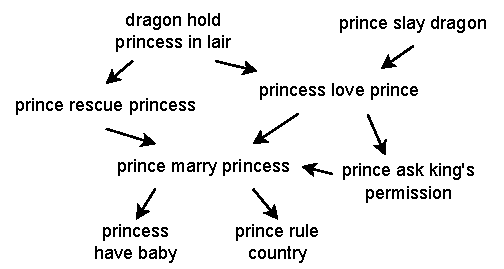
\includegraphics[width=0.7\columnwidth]{chapter2/pictures/plot_graph.pdf}
    \caption{Plot graph for the sentence: \emph{``the princess loves the prince''} \citep{mcintyre2010plot}.}
    \label{fig:plot_graph}
\end{figure}

\subsection{Machine Learning-based Models}

Contrary to the rule-based {\asg} systems presented in \autoref{sub:structural_models} and \autoref{sub:planning_based_models}, machine learning-based models rely on probabilistic strategies. In recent years, the vast majority of machine learning-based models have been employing language models. In the next section, we provide an overview of the evolution of language models. We review the models specific to {\asg} later, in \autoref{sub:neural_asg}.

\section{Language Models}
\label{sec:language_models}

Language models are probabilistic models of natural language. More precisely, their function is to estimate the probability distribution of the next word for a given sequence of words. The first developed language models were called statistical language models, for they relied on statistical estimation techniques applied to textual data. In the 2010s, language models relying on neural architectures started to achieve state-of-the-art performance in many Natural Language Processing (\nlp) tasks (\eg\ machine translation, named entity recognition, semantic role labeling, question answering, etc.), and they have now become omnipresent in \nlp\ research topics, including \asg. In this section, we will describe the most noteworthy advances in the development of language models, from statistical language models to the current state-of-the-art models, which are called Large Language Models ({\llm}s).

\subsection{Statistical Language Models}

\subsubsection{Definitions}
Statistical Language Models (\slm) attempt to capture regularities of natural language for the purpose of improving the performance of various natural language applications \citep{rosenfeld2000two}. Before the advent of neural models, they were commonly used for machine translation, document classification, information retrieval, and many other tasks.

A \slm\ is, at its core, a probability distribution $P(s)$ over all possible sentences $s$. \slm s were usually used in the context of a Bayes' classifier, where they could play the role of either the prior or the likelihood function. For instance, in automatic speech recognition, given an acoustic signal $a$, the goal is to find the sentence $s^\star$ that is most likely to have been spoken. With a Bayesian framework, the solution is:

\[ s^\star = \argmax_s P(s \mid a) = \argmax_s \left( P(a \mid s) \cdot P(s) \right) \]

where the language model $P(s)$ plays the role of the \emph{prior}.

By contrast, in document classification, given a document $d$, the goal is to find the most probable class $c^\star$. Typically, for each class $c$, we have a corresponding language model $P_c(d)$. The solution is then:

\[ c^\star = \argmax_c P(c \mid d) = \argmax_c \left( P(d \mid c) \cdot P(c) \right) = \argmax_c \left( P_c(d) \cdot P(c) \right) \]

where the language models $P_c(d)$ play the role of the \emph{likelihood}.

The quality of a given \slm\ is commonly assessed using the \emph{cross-entropy} of a new data sample.

\begin{defi}{Cross-entropy (\slm)}{crossentropy_slm}
    Let $P$ be a statistical language model and $X = \{ w_1, \dots, w_N \}$ a sentence of $N$ words.\\
    The cross-entropy of $X$ is defined by:
    \[ \mathrm{CE}(X) \coloneqq \frac{1}{N} \sum_i - \log_2 P(w_i) . \]
\end{defi}

Cross-entropy can be interpreted as the average number of bits that would be required to encode the sample data using an optimal coder. Assuming the data is generated by a random process, a perfect model would have the lowest cross-entropy possible. Thus, we generally aim to decrease model cross-entropy, as it is used as an inverse proxy for model quality.

In practice, the performance of a \slm\ is often reported in terms of \emph{perplexity}.

\begin{defi}{Perplexity (\slm)}{perplexity_slm}
    Let $P$ be a statistical language model and $X = \{ w_1, \dots, w_N \}$ a sentence of $N$ words.\\
    The perplexity of $X$ is defined by:
    \[ \mathrm{PPL}(X) \coloneqq 2^{\mathrm{CE}(X)} = 2^{\frac{1}{N}\sum_i - \log_2 P(x_i)} . \]
\end{defi}

Perplexity can be interpreted as the average branching factor of the language according to the model, \ie, the weighted average number of choices for each word. As perplexity becomes lower, the model tends to make more accurate predictions, although there have been occurrences in the literature of negative correlations between perplexity and error rate \citep{chen1998evaluation}.

A variety of \slm\ techniques has been developed, such as $n$-gram models, decision tree models, context-free grammars, exponential models, adaptive models, etc. We will here only describe $n$-gram models, which were by far the most popular forms of \slm . A more detailed account can be found in \citet{rosenfeld2000two}. 

\subsubsection{$n$-gram Models}
For a sentence $s$ composed of words $w_1, \dots, w_l$, we can express its probability $P(s)$ by:

\begin{align*}
    P(s)    & = P(w_1) P(w_2 \mid w_1) P(w_3 \mid w_1, w_2) \dots P(w_l \mid w_1, \dots, w_{l-1}) \\
            & = P(w_1) \prod_{i=2}^l P(w_i \mid w_1, \dots, w_{i-1}) .
\end{align*}

The intuition of the $n$-gram model is that instead of computing the probability of a word given all its predecessors, we assume that the probability depends only on the $n-1$ previous words. For instance, for $n=3$, we assume that:

\[ P(w_i \mid w_1, \dots, w_{i-1}) \approx P(w_i \mid w_{i-2}, w_{i-1}) . \]

The value of $n$ trades off the variance of the estimate against its bias. Incidentally, the trigram assumption ($n=3$) has been shown to work well in practice \citep{goodman2001bit} and is a common choice with large training corpora, while bigrams ($n=2$) are used with smaller ones. Trigram probabilities $C(w_{i-2}, w_{i-1}, w_i)$ are usually estimated from counts on a training corpus, and similarly for bigram probabilites $C(w_{i-2}, w_{i-1})$. Then, we can approximate:

\[ P(w_i \mid w_{i-2}, w_{i-1}) \approx \frac{C(w_{i-2}, w_{i-1}, w_i)}{C(w_{i-2}, w_{i-1})} . \]

A glaring weakness of $n$-gram models is that this approximation is very noisy, since many $n$-grams do not appear in the training data. The probability of unseen $n$-grams therefore defaults to 0, which can severely impede model performance. To mitigate this phenomenon, smoothing strategies were introduced \citep{chen2000survey}. For instance, Kneser-Ney smoothing \citep{kneser1995improved}, commonly seen as the overall best smoothing strategy, accounts for unseen $n$-grams by subtracting a fixed number $D$ from all $n$-gram counts. It then estimates the probability of an unseen $n$-gram by interpolating the probabilities of all lower-order $n$-grams: if any $k$-gram of a sequence was seen in the corpus, the sequence will have a non-zero probability.

Several other techniques have been developed to improve $n$-gram models, such as skipping, clustering, caching, sentence mixture, etc. \citep{goodman2001bit}.

A few attempts to use $n$-gram models for story generation were made, with limited success. \citet{swanson2009comparison} describe a system that takes an input sentence from a user and searches in a database for a sentence that continues the story. Specifically, the retrieval procedure uses a context bigram model. \citet{limpanadusadee2014text} evaluate the performance of $n$-gram models for storytelling sentence generation in Thai: 3- or 4- word sentence generation yielded between 40\% and 100\% accuracy, dropping to as low as 10\% for 6-word sentences.

\subsection{Neural Language Models}

\subsubsection{A Brief History of Neural Networks}

Neural networks are algorithms used for machine learning, which is defined as the field of study that gives computers the ability to learn without being explicitly programmed \citep{samuel1959machine}. Neural networks take inspiration from the human brain's architecture, where a neuron's computations involve a weighted sum of its input values, to which a nonlinear function is applied. The first neural network model was proposed by \citet{mcculloch1943logical}, who proved that any finite logical expression can be realized by a network of artificial neurons. Then, \citet{hebb1949organization} coined the term ``connectionism'' and described a method of updating synaptic weights, as well as other contributions which are now implemented in neural network models, at least to some degree. \citet{rosenblatt1958perceptron} defined a neural network structure called the perceptron, which is considered a landmark in the history of neural networks and laid the groundwork for both supervised and unsupervised learning. \citet{widrow1960adaptive} introduced \textsc{Adaline}, a neural network model with a different learning algorithm from the perceptron, of which an extension is used in today's backpropagation networks. Neural networks were then forgotten for a few decades, in part due to a campaign that discredited their potential \citep{minsky1969introduction}. In the 1980s, several events sparked a regain of interest in neural networks: \citet{hopfield1982neural} presented recurrent artificial neural networks serving as content-adressable memory systems, \citet{rumelhart1985learning} rediscovered the backpropagation algorithm (first discovered by \citet{werbos1974beyond}) and \cite{le1989handwritten} proposed the LeNet network for hand-written digit recognition. As neural networks became deeper, the backpropagation algorithm became slower and had a glaring weakness: it suffered from the vanishing gradient problem. This was eventually solved when multiple studies (\eg\ \citet{nair2010rectified}, \citet{glorot2011deep}) advised to use the rectified linear unit (\textsc{ReLU}) activation function. The early 2010s then saw a significant rise in usage of neural networks, helped by a growing abundance of training data and an increased availability of both computational power and graphics processing units.

\subsubsection{Basic Notions}
\begin{defi}{Neural Network}{neural_network}
A neural network is a machine learning architecture which maps a vectorized input $\mathbf{x}$ to a vectorized output $\mathbf{y}$ through a parameterized function $f$:

\[ \hat{\mathbf{y}} = f(\mathbf{x}, \theta) , \]

where $\hat{\mathbf{y}}$ is the predicted output produced by the function $f$ with parameters $\theta$.
\end{defi}

The building block of neural networks is the \emph{neuron}, whose inputs $x_i$ are weighted by learned parameters $w_i$ and linearly combined with a bias $b$ before the application of a non-linear function. The first neuron algorithm to be implemented on real hardware was the perceptron, proposed by \citet{rosenblatt1958perceptron}.

\begin{defi}{Perceptron}{perceptron}
The perceptron is an an algorithm for learning a binary classifier called a threshold function: it maps its input $\mathbf{x}$ (a real-valued vector) to an output value $f(\mathbf{x})$ (a single binary value):

\[ f(\mathbf{x}) = \theta (\mathbf{w} \cdot \mathbf{x} + \mathbf{b}) , \]

where $\theta$ is the Heaviside step-function, $\mathbf{w}$ a vector of real-valued weights and $\mathbf{b}$ a bias vector.
\end{defi}

Following the introduction of the perceptron, different types of architectures for neural networks have been proposed, such as the \emph{feed-forward neural network}, the \emph{convolutional neural network} (\cnn) and the \emph{recurrent neural network} (\rnn).

\paragraph{Feed-Forward Neural Network.}

The most basic type of neural network is the feed-forward neural network, where neurons are arranged in multiple layers. Each neuron receives as inputs the outputs from the neurons of the previous layer. For a \emph{fully-connected} feed-forward neural network containing two hidden layers, the function can be summarized as:

\begin{align*}
    \hat{\mathbf{y}} & = \sigma(\mathbf{W}_3 \, \mathbf{h}_2 + \mathbf{b}_3 ) \\
    \mathbf{h}_2     & = f_2(\mathbf{W}_2 \, \mathbf{h}_1 + \mathbf{b}_2 ) \\
    \mathbf{h}_1     & = f_1(\mathbf{W}_1 \, \mathbf{x} + \mathbf{b}_1 ) ,
\end{align*}

where 

\begin{itemize}[nolistsep]
    \item $\mathbf{x}$ is the input vector,
    \item $\mathbf{h}_1$ and $\mathbf{h}_2$ are the first and second layers respectively,
    \item $\hat{\mathbf{y}}$ is the output vector,
    \item $f_1$ and $f_2$ are non-linear functions (\eg\ the sigmoid function, the hyperbolic tangent or the rectified linear unit (\textsc{ReLU}))
    \item the $\mathbf{W}_i$ and $\mathbf{b}_i$ for $i \in \{1,2,3\}$ are the learned weights,
    \item $\sigma$ is the softmax function defined as:
        \begin{align*}
        \sigma \colon \mathbb{R}^n & \rightarrow \mathbb{R}^n \\
        \mathbf{z} & \mapsto \left( \frac{e^{(z_j)}}{\sum_{k=1}^K e^{(z_k)}} \right)_{j \in \{1, \dots, n\}} . \\
        \end{align*}
\end{itemize}

\begin{figure}[h!]
    \centering
    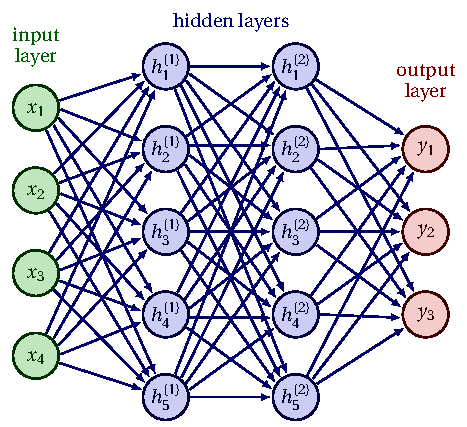
\includegraphics[width=0.55\columnwidth]{chapter2/pictures/neural_network.pdf}
    \caption{A fully-connected feed-forward neural network \citep{neutelingsNeuralNetworks2021}.}
    \label{fig:fcffnn}
\end{figure}

A corresponding visual example can be seen on \autoref{fig:fcffnn}.

\paragraph{Convolutional Neural Networks (\cnn).}
\cnn s, like feed-forward neural networks, consist of an input layer, hidden layers and an output layer. In \cnn s, the hidden layers include one or more layers that perform convolutions, \ie, layers that perform a dot product of the convolution kernel with the layer's input matrix. As the convolution kernel slides along the input matrix for the layer, the convolution operation generates a feature map, which in turn contributes to the input of the next layer, as shown on \autoref{fig:cnn}. Usually, the convolutional layers are followed by other layers, \eg\ pooling layers, fully-connected layers, and normalization layers. While \cnn s have sometimes been used for natural language processing tasks, they are mainly used in computer vision settings, \eg\ for image classification or object recognition.

\begin{figure}[h!]
    \centering
    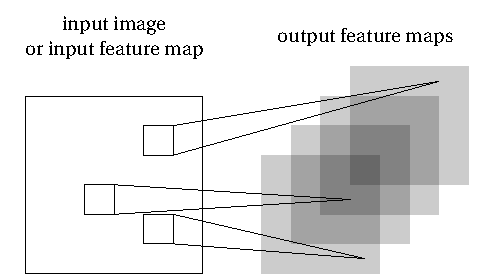
\includegraphics[width=0.5\columnwidth]{chapter2/pictures/convolutional_neural_network.pdf}
    \caption{A layer of a convolutional neural network \citep{stutzIllustratingConvolutionalNeural2020}.}
    \label{fig:cnn}
\end{figure}

\paragraph{Recurrent Neural Networks (\rnn).}
\rnn s are bi-directional neural networks: the output from some nodes can affect subsequent input to the same nodes. \rnn s can use internal states to process arbitrary sequences of inputs, which makes them well-suited for tasks related to natural language processing. \rnn s typically share parameters acorss each layer of the nertwork and leverage backpropagation through time for their training procedure.

\begin{figure}[h!]
    \centering
    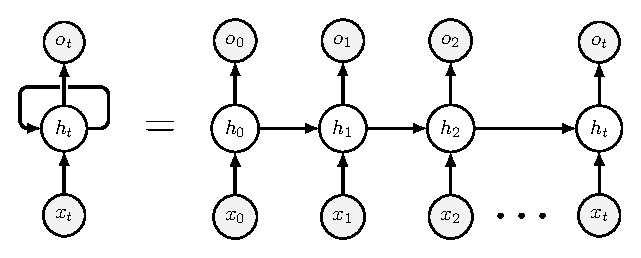
\includegraphics[width=0.8\columnwidth]{chapter2/pictures/tikz_rnn.pdf}
    \caption{A fully-recurrent neural network \citep{user1217992019tikz}.}
    \label{fig:tikz_rnn}
\end{figure}

A basic fully-recurrent neural network (shown on \autoref{fig:tikz_rnn}) can be described by the two following formulas:

\begin{align*}
    \mathbf{h}_{t+1} & = f\left( \mathbf{W}_x \cdot \mathbf{x}_t + \mathbf{W}_h \cdot \mathbf{h}_t + \mathbf{b}_h \right) \\
    \mathbf{o}_{t+1} & = f\left( \mathbf{W}_o \cdot \mathbf{h}_t + \mathbf{b}_o \right),
\end{align*}

where
\begin{itemize}[nolistsep]
    \item $\mathbf{x}_t$ is the input vector at time $t$,
    \item $\mathbf{h}_t$ is the hidden state vector at time $t$,
    \item $\mathbf{o}_t$ is the output vector at time $t$,
    \item the $\mathbf{W}$'s and $\mathbf{b}$'s are weight matrices and bias vectors parameters learned during training and shared across time steps.
\end{itemize}

However, the high depth of {\rnn}s can make them subject to the vanishing gradient problem, where the gradients computed for updating the weights would have near-zero values. To solve this issue, different architectures were proposed, such as the \emph{long short-term memory} (\lstm) network.

\paragraph{Long Short-Term Memory (\lstm).}
An {\lstm} network \citep{hochreiter1997long, sundermeyer2012lstm} is composed of multiple units, with each unit containing a cell, an input gate, an output gate and a forget gate. The three gates control the information flow into and out of the cell, and the cell retains values for arbitrarily long periods of time. Forget gates use a coefficient between 0 and 1 to decide at which rate information from a prior state should be discarded {\wrt}\ the present input. Using the same mechanism as forget gates, input gates determine which new pieces of information to store in the existing state, and output gates regulate the information to output. This architecture enables {\lstm} networks to  retain valuable long-term dependencies.

Formally, an \lstm\ network (see \autoref{fig:lstm}) computes a mapping from an input sequence $\mathbf{X} = (\mathbf{x}_1, \dots, \mathbf{x}_T)$ to an output sequence $\mathbf{Y} = (\mathbf{y}_1, \dots, \mathbf{y}_T)$ using the following equations iteratively from $t = 1$ to $T$:
\begin{align*}
    \mathbf{f}_t & = \sigma_g (\mathbf{W}_f \, \mathbf{x}_t + \mathbf{U}_f \, \mathbf{h}_{t-1} + \mathbf{b}_f) \\
    \mathbf{i}_t & = \sigma_g (\mathbf{W}_i \, \mathbf{x}_t + \mathbf{U}_i \, \mathbf{h}_{t-1} + \mathbf{b}_i) \\
    \mathbf{o}_t & = \sigma_g (\mathbf{W}_o \, \mathbf{x}_t + \mathbf{U}_o \, \mathbf{h}_{t-1} + \mathbf{b}_o) \\
    \Tilde{\mathbf{c}}_t & = \tanh (\mathbf{W}_o \, \mathbf{x}_t + \mathbf{U}_c \, \mathbf{h}_{t-1} + \mathbf{b}_c) \\
    \mathbf{c}_t & = \mathbf{f}_t \odot \mathbf{c}_{t-1} + \mathbf{i}_t \odot \Tilde{\mathbf{c}}_t \\
    \mathbf{h}_t & = \mathbf{o}_t \odot \tanh(\mathbf{c}_t) , \\
    \mathbf{y}_t & = \mathbf{h}_t
\end{align*}
where
\begin{itemize}[nolistsep]
    \item $\mathbf{x}_t$ is the input vector,
    \item $\mathbf{f}_t$ is the forget gate's activation vector,
    \item $\mathbf{i}_t$ is the input gate's activation vector,
    \item $\mathbf{o}_t$ is the output gate's activation vector,
    \item $\mathbf{h}_t$ is the hidden state vector,
    \item $\mathbf{y}_t$ is the output vector,
    \item $\Tilde{\mathbf{c}}_t$ is the cell input activation vector,
    \item $\mathbf{c}_t$ is the cell state vector,
    \item the $\mathbf{W}$'s, $\mathbf{U}$'s and $\mathbf{b}$'s are weight matrices and bias vectors parameters learned during training,
    \item $\sigma_g$ is the sigmoid function.
\end{itemize}

\begin{figure}[h!]
    \centering
    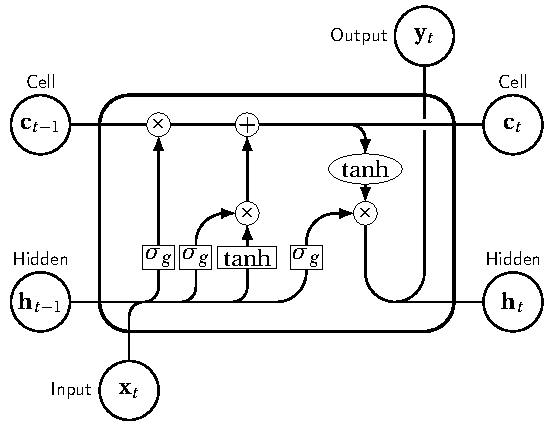
\includegraphics[width=0.75\columnwidth]{chapter2/pictures/lstm_cell.pdf}
    \caption{An LSTM cell \citep{vAnswerHowDraw2018}.}
    \label{fig:lstm}
\end{figure}

\subsubsection{Neural Network Training}
In order to learn the best parameters, one needs to \emph{train} a neural network. It is typically done through the minimization of a loss function over a training set, typically with a gradient-based method \citep{goldberg2016primer}. Most such methods repeatedly compute an estimate of the error over the dataset, then compute the gradient with respect to the error, and update the parameters by moving them in the direction opposite to the gradient.

\paragraph{Loss Functions.}
A loss function $L$ assigns a numerical score $L(\hat{\mathbf{y}}, \mathbf{y})$ which estimates the error between the network's output $\hat{\mathbf{y}}$ and the true expected output $\mathbf{y}$. The loss function should be bounded from below, with the minimum attained only for cases where the network's output is the true expected output.

In regression settings, a common loss is the \emph{mean squared error} (\textsc{MSE}), defined by:

\[ \textrm{MSE}(\hat{\mathbf{y}}, \mathbf{y}) = \frac{1}{n} \sum_{i=1}^n (\hat{y}_i, y_i)^2 . \]

The variability of the gradient of the \textsc{MSE} loss is beneficial to the fast convergence and high accuracy of the model, but makes it very sensitive to outliers. 

For classification settings, which are more common in \nlp, the categorical cross-entropy loss (or negative log-likelihood) is typically used. It is defined by:

\[ L_\textrm{cross-entropy}(\hat{\mathbf{y}}, \mathbf{y}) = - \sum_i y_i \log (\hat{y}_i) , \]

where $\mathbf{y}$ is the true multinomial distribution over the labels $1, \dots, n$ and $\hat{\mathbf{y}}$ is the network's output after the softmax activation function, \ie, the class membership conditional distribution: $\hat{y}_i = P(y = i \mid \mathbf{x})$.

The output of this loss provides a probabilistic interpretation and the softmax function makes it quite stable, but it can be sensitive to imbalanced datasets, where the number of samples for each class is not equal.

We refer the reader to \citet{wang2020comprehensive} for a more comprehensive discussion on loss functions in machine learning.

\paragraph{Optimization Algorithms.}
Early attempts at minimizing the loss function (\eg\ \citep{rumelhart1985learning}) used the gradient descent algorithm, in which the weights are iteratively updated according to the following formula:

 \[ \mathbf{W}_{t+1} = \mathbf{W}_t - \gamma \nabla L(\hat{\mathbf{y}}, \mathbf{y}) , \]

 where $\gamma$ is an adaquately chosen parameter. Under sufficient regularity assumptions, when the initial estimate $W_0$ is close enough to the optimum, and when $\gamma$ is sufficiently small, the gradient descent achieves linear convergence \citep{dennis1996numerical}.

 Since then, numerous other approaches have been proposed: stochastic gradient descent, batch gradient descent, \textsc{Adagrad} \citep{duchi2011adagrad}, \textsc{RMSProp} \citep{tieleman2012rmsprop}, \textsc{Adam} \citep{kingma2015adam}, etc.

\subsubsection{First Neural Models}
The goal of statistical language modeling is to learn the joint probability function of sequences of words in a language, where words are modeled by discrete random variables. \citet{bengio2000neural} observed that this objective is intrinsically difficult because of the curse of dimensionality: it is likely that word sequences encountered by the model will not have been seen during training. They proposed a recurrent neural model that learned a distributed representation for words along with the probability distribution of word sequences: in particular, the model associates with each word in the vocabulary a \emph{feature vector}, {\ie}, a real-valued vector in $\mathbb{R}^m$ where $m$ is a chosen size. The idea was further refined by \citet{mikolov2010recurrent}, and showed significant improvements in performance compared to $n$-gram models in terms of perplexity. While feed-forward neural networks had also been tested for language modeling \citep{xu2000can}, \rnn-based models had an inherent advantage in their ability to process sequence data of variable lengths, and the sharing of parameters across layers reduced the number of computations compared to feed-forward neural networks \citep{jing2019survey}.

\subsubsection{Static Word Embeddings}
\citet{mikolov2013efficient} proposed the \wvec\ architecture for computing continuous vector representations of words. Contrary to previous count-based approaches such as one-hot encoding, the \wvec\ approach allows for language models to learn high-quality word vectors from datasets containing billions of words, with millions of words in the vocabulary. In particular, it was shown that the computed representations of words displayed multiple degrees of similarity. Two variations were proposed: continuous bag of words (\cbow) and Skip-gram (see \autoref{fig:word2vec}). The main motivation behind those new architectures was to reduce computational complexity: a simpler model would be trained to produce word representations that could then be used by more complex {\rnn}-based models. In \cbow, the context word vectors are projected into the same position in order to produce an averaged vector, which is used to predict the target word. In Skip-gram, the task in reversed: the model is shown the target word and has to predict the context words. They show that the learned word vectors from their models outperform the previous state-of-the-art on relational similarity tasks. 

\begin{figure}[h]
    \centering
    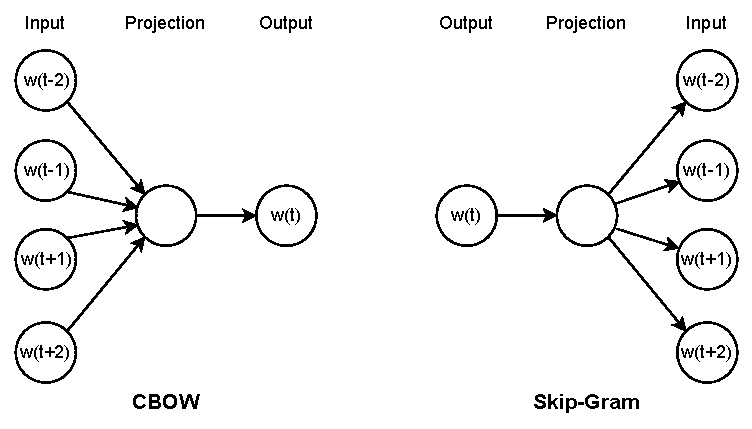
\includegraphics[width=\columnwidth]{chapter2/pictures/word2vec.pdf}
    \caption{CBOW and Skip-gram architectures \citep{mikolov2013efficient}.}
    \label{fig:word2vec}
\end{figure}

\citet{mikolov2013distributed} improved \wvec\ through the use of multiple strategies: hierarchical softmax (which allows for evaluation of only $\log_2(W)$ output nodes instead of $W$ nodes for obtaining the probability distribution), subsampling of frequent words (deleting frequent words from the training corpus), and negative sampling (updating only a limited number of incorrect words for each training instance).

Other static word embeddings built upon the \wvec\ appraoch. \glove\ embeddings \citep{pennington2014glove} combine the advantages of the two major model
families in the literature: global matrix factorization and local context window
methods. They leverage statistical information by training only on the nonzero elements in a word-word co-occurrence matrix, rather than on the entire sparse matrix or on individual context windows in a large corpus. \ftext\ embeddings \citep{bojanowski2017enriching} are based on the Skip-gram model, where each word is represented as a bag of character $n$-grams. A vector representation is associated to each character $n$-gram and words are represented as the sum of these representations. 

\subsubsection{\rnn\ Encoder-Decoder}
While {\rnn}s are powerful and flexible, they could only be applied to tasks where inputs and outputs are of fixed lengths. However, many {\nlp} tasks, such as machine translation, involve variable-length inputs and outputs. To solve this issue, \citet{cho2014learning} and \citet{sutskever2014sequence} introduced the \emph{Encoder-Decoder} framework, also called \emph{Sequence-to-sequence (\seqseq)} framework. This architecture consists of two \rnn s: the first \rnn\ encodes a sequence of symbols into a fixed-length vector representation, and the second \rnn\ decodes that representation into another sequence of symbols.

Formally, the Encoder-Decoder can be described as follows: an encoder reads the input sentence $\mathbf{x} = (x_1, \dots, x_T)$ into a vector $c$. Commonly, a \rnn\ is used such that

$$ h_t = f(x_t, h_{t-1}) \quad \text{and} \quad c = q(h_1, \dots, h_T),$$

where $h_t$ is the hidden state at time $t$, and $f$ and $q$ are nonlinear functions. For instance, \citet{sutskever2014sequence} used an \lstm\ as $f$ and $q(h_1, \dots, h_T) \coloneqq h_T$.

Then, the decoder  is trained to predict the next word $y_{t^\prime}$ given the context vector $c$ and the previously predicted words $y_1, \dots, y_{t^\prime - 1}$, \ie, it defines a probability over the output sequence $\mathbf{y}$ by decomposing the joint probability into the ordered conditionals:

\[ p \left(y_1, \dots, y_{T_y} \mid x_1, \dots, x_{T_x}\right) = \prod_{t=1}^{T_y} p\left(y_t \mid c, y_1, \dots, y_{t-1} \right) . \]

With an \rnn, each conditional probability is modeled as

\[ \prod_{t=1}^{T_y} p\left(y_t \mid c, y_1, \dots, y_{t-1} \right) = g\left(y_{t-1}, s_t, c \right) , \]

where $g$ is a nonlinear function that outputs the probability of $y_t$, and $s_t$ is the hidden state of the \rnn.

In particular, \citet{sutskever2014sequence} showed that a large deep LSTM Encoder-Decoder model with limited vocabulary and few assumptions about problem structure was able to outperform statistical language models for machine translation tasks. 

\subsubsection{Attention Mechanism}
\citet{bahdanau2014neural} conjectured that the Seq2seq framework's encoding of the input sequence into a fixed-length vector was a bottleneck for performance improvement, since it may limit its ability to process long sentences \citep{cho2014learning}. Thus, they extended the architecture by allowing the model to automatically soft-search for parts of the input sequence that are relevant to predicting a target word, which would later be called the \emph{attention mechanism}. The new model they propose for machine translation consists of a bidirectional \rnn\ as an encoder and a decoder that emulates searching through a source sentence when decoding a translation.

The encoder is supposed to annotate each word by summarizing both the preceding and following words, hence they choose a bidirectional RNN. The forward RNN $\overrightarrow{f}$ reads the input sequence $(x_1, \dots, x_{T_x})$ from left to right and computes a sequence of forward hidden states $(\overrightarrow{h}_1, \dots, \overrightarrow{h}_{T_x})$. Conversely, the backward RNN $\overleftarrow{f}$ reads the input from right to left and computes backward hidden states $(\overleftarrow{h}_1, \dots, \overleftarrow{h}_{T_x})$. The annotation $\mathbf{h}_j$ for each word $x_j$ is obtained by concatenation of both hidden states:

\[ h_j = \left[ {\overrightarrow{h}_j}^\mathsf{T} \, ; \, {\overleftarrow{h}_j}^\mathsf{T} \right]^\mathsf{T} . \]

In the decoder, each conditional probability for a word $y_i$ is defined as

\[ p\left(y_i \mid y_1, \dots, y_{i-1}, c_i \right) = g\left(y_{i-1}, s_i, c_i \right) , \]

where $g$ is a non-linear (potentially multi-layered) function and $s_i$ is the \rnn\ hidden state for time $i$ computed by

\[ s_i = f\left(s_{i-1}, y_{i-1}, c_i\right) . \]

Unlike in the RNN Encoder-Decoder, there is a context vector $c_i$ for each word $y_i$.

$c_i$ is computed as a weighted sum of the annotations $(h_1, \dots, h_{T_x})$ produced by the encoder:

\[ c_i = \sum_{j=1}^{T_x} \alpha_{ij} h_j \qquad \text{where} \qquad \alpha_{ij} = \frac{\exp(e_{ij})}{\sum_{k=1}^{T_x} \exp(e_{ik})} \qquad \text{where} \qquad e_{ij} = a(s_{i-1}, h_j) \]

is an alignment model which scores how well the inputs around position $j$ and the output at position $i$ match. The score is based on the previous hidden state $s_{i-1}$ and the $j$-th annotation $h_j$ of the input.

\citet{bahdanau2014neural} originally chose to parameterize $a$ as a feedforward neural network jointly trained with the rest of the architecture:

\[ a(s_{i-1}, h_j) = v_a^\mathsf{T} \tanh \left(W_a [s_{i-1} ; h_i] \right) . \]

Other alignment scores have been proposed:
\begin{enumerate}[nolistsep]
    \item Content-based \citep{graves2014neural}: $a(s_{i-1}, h_j) = \cos(s_{i-1}, h_j)$;
    \item Location-based \citep{luong2015effective}: $\alpha_{ij} = \mathrm{softmax}(W_a s_{i-1})$ (no dependency on the source position);
    \item General \citep{luong2015effective}: $a(s_{i-1}, h_j) = s_{i-1}^\mathsf{T} W_a h_j$;
    \item Dot-product \citep{luong2015effective}: $a(s_{i-1}, h_j) = s_{i-1}^\mathsf{T} h_j$;
\end{enumerate}

The context vector $c_i$ can be understood as an expected annotation with $\alpha_{ij}$ being the probability that $y_i$ is aligned with $x_j$. Meanwhile, $\alpha_{ij}$ reflects the importance of the annotation $h_j$ with respect to the previous hidden state $s_{i-1}$ in deciding the next $s_i$ and generating the next word $y_i$, \ie, it reflects how much the decoder should pay ``attention'' to the annotation.

\subsubsection{Contextual Embeddings}

\citet{peters-etal-2018-deep} introduce {\elmo} (Embeddings from Language Models), a new type of deep contextualized word representation that is able to model both (1) complex characteristics of word use ({\eg}\ syntax and semantics), and (2) how these uses vary across linguistic contexts ({\ie}, to model polysemy). They demonstrate that this representation can be easily integrated into existing models, and significantly improves the state of the art in every considered case across a range of challenging language understanding problems.

{\elmo} is designed as a task specific combination of the intermediate layer representations of a bidirectional language model (biLM). For each token $t_k$, a $L$-layer biLM computes a set of $2L + 1$ representations: the initial token embedding $x_k$, and the respectively forward and backward embeddings $\overrightarrow{h}_{k,j}$ and $\overleftarrow{h}_{k,j}$ for each layer $j$.

Let $h_{k,0} \coloneqq x_k$ and $h_{k,j} \coloneqq \left[ \overrightarrow{h}_{k,j} ; \overleftarrow{h}_{k,j} \right]$. {\elmo} is defined as a weighted average of all biLM layers:

\[ \elmo_k \coloneqq \gamma^{\mathrm{task}} \sum_{j=0}^L s^{\mathrm{task}}_j h_{k,j} , \]

where the $s^{\mathrm{task}}_j$ are softmax-normalized weights and
the scalar parameter $\gamma^{\mathrm{task}}$ allows the task model to scale the entire {\elmo} vector.

Through extensive experiments, they demonstrate that {\elmo} representations work extremely well in practice. They first show that they can be easily added to existing models for six diverse language understanding problems, such as question answering and sentiment analysis, and that the addition of {\elmo} representations alone significantly improves the state of the art in every case, including up to 20\% relative error reductions. 

\subsection{The Transformer Era} 

The introduction of the transformer architecture in the landmark paper ``Attention Is All You Need'' \citep{vaswani2017attention} marked a notable shift in \nlp, as transformers would become the foundation of all future advances in the development of language models. Departing from the usual \rnn-based or rarer \cnn-based models, they proposed an auto-regressive architecture that relied entirely on attention mechanisms. Notably, the transformer achieved new state of the art performance in the WMT 2014 tasks. 

\begin{figure}[!h]
    \begin{minipage}{0.6\columnwidth}
        \centering
        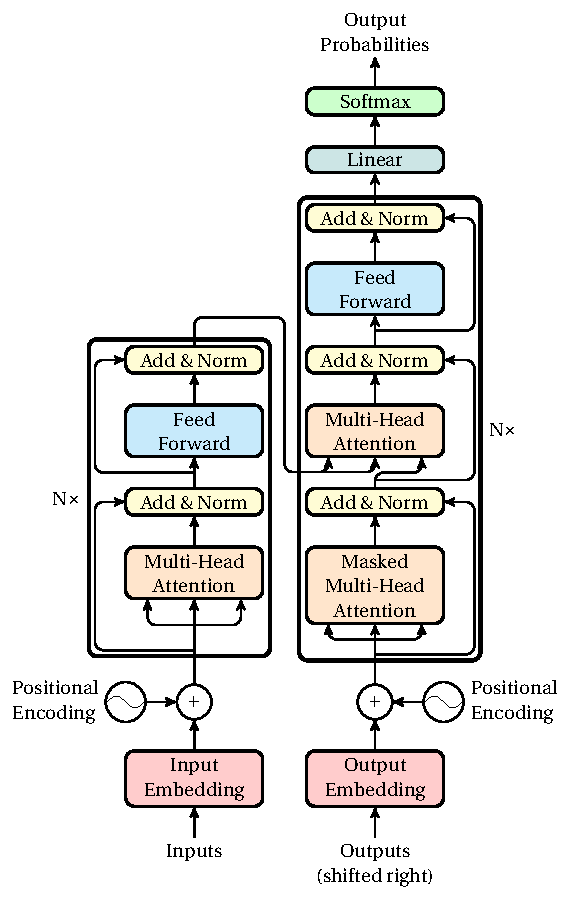
\includegraphics[width=\textwidth]{chapter2/pictures/transformer.pdf}
        \caption{The transformer architecture \citep{vaswani2017attention}.}
        \label{fig:transformer}
    \end{minipage}
    \hspace{3em}
    \begin{minipage}{0.3\columnwidth}
        \centering
        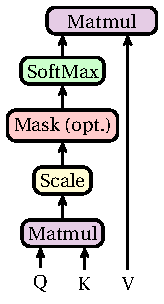
\includegraphics[width=0.6\columnwidth]{chapter2/pictures/scaled_dot_product_attention.pdf}
        \caption{Scaled dot-product attention \citep{vaswani2017attention}.}
        \label{fig:scaled_dot_product_attention}
        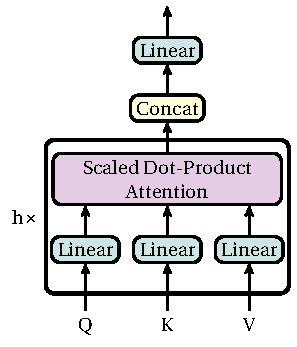
\includegraphics[width=\columnwidth]{chapter2/pictures/multihead_attention.pdf}
        \caption{Multi-head attention \citep{vaswani2017attention}.}
        \label{fig:multi_head_attention}
    \end{minipage}
\end{figure}

\subsubsection{Encoder and Decoder Stacks}
The transformer, like the \rnn\ encoder-decoder, is composed of an encoder and a decoder (see \autoref{fig:transformer} for an illustration).
The encoder consists of $N$ stacks of identical encoder layers containing two sub-layers: a multi-head self-attention mechanism and a feed-forward network. The decoder contains the same sub-layers and inserts a third sub-layer which performs multi-head attention over the output of the encoder stack. Also, this sub-layer is masked to prevent positions from attending to subsequent positions, \ie, to ensure that predictions for position $i$ depend only on positions less than $i$. Finally, residual connections are employed around each sub-layer, followed by layer normalization.

\subsubsection{Scaled Dot-Product Attention}
The transformer uses a particular attention mechanism called scaled dot-product attention (see \autoref{fig:scaled_dot_product_attention}), where the input consists of queries and keys of dimension $d_k$ and values of dimension $d_v$. Queries, keys, and values are packed together into matrices $Q$, $K$, and $V$, and the output is computed as follows:

\[ \mathrm{Attention}(Q, K, V) \coloneqq \mathrm{softmax} \left( \frac{Q K^\mathsf{T}}{\sqrt{d_k}} \right) V .\]

The main advantage of scaled dot-product attention over previous attention functions is that it is faster, more space-efficient, and can be implemented using highly-optimized matrix multiplication code. 

\subsubsection{Multi-Head Attention}
Instead of performing a single attention function with large $d_\textrm{model}$ dimensional queries, keys, and values, matrices are projected $h$ times with different, learned linear projections to $d_k$, $d_k$, and $d_v$ dimensions respectively (see \autoref{fig:multi_head_attention}). This multi-head attention strategy allows the model to jointly attend to information from different representation subspaces at different positions, since attention operations can be performed in parallel. Output values are then concatenated and once again projected. Formally:

\[ \mathrm{MultiHead}(Q, K, V) \coloneqq \mathrm{Concat}\left(\mathrm{head}_1, \dots, \mathrm{head}_h \right) W^O , \]

where $\mathrm{head}_i \coloneqq \mathrm{Attention} \left( QW_i^Q, KW_i^K, VW_i^V \right)$.

In practice, due to the reduced dimension of each head, the total computational cost is similar to that of a single-head attention with full dimensionality.

\subsubsection{Positional Encoding}
Positional encoding is an important measure taken so that the transformer can make use of the order of the sequence without recurrence or convolution. It consists in the injection of some information about the relative or absolute position of tokens in the sequence:

\begin{align*}
\mathrm{PE}_{(\mathrm{pos}, 2i)} & \coloneqq \sin \left( \frac{\mathrm{pos}}{10000^{\frac{2i}{d_\mathrm{model}}}} \right) \\
\mathrm{PE}_{(\mathrm{pos}, 2i+1)} & \coloneqq \cos \left( \frac{\mathrm{pos}}{10000^{\frac{2i}{d_\mathrm{model}}}} \right) ,
\end{align*}

where $\mathrm{pos}$ is the position and $i$ the dimension.

This function was chosen as it was hypothesized that the model would easily learn to attend by relative positions since, for any fixed offset $k$, $\mathrm{PE}_{\mathrm{pos}+k}$ can be represented as a linear function of $\mathrm{PE}_{\mathrm{pos}}$.

In practice, for each position in the sentence, positional embedding is computed as a $d_\textrm{model}$-dimensional vector which is added to the corresponding word embedding vector.

\subsection{Pre-trained Language Models} 
\label{sub:pretrained_language_models}

Following the introduction of the transformer architecture, multiple language models based on transformers were proposed, with each one of them achieving new state-of-the-art performance. We can separate them into three different types: decoder-only, encoder-only, and encoder-decoder models, which respectively use either only the decoder part of the transformer architecture, only the encoder part, or both.

\subsubsection{Decoder Models}

In decoder models, for each word from the input sentence, the attention layers can only access the words positioned before it. These models are often called \emph{auto-regressive} models. The main pretraining objective of decoder models is usually to predict the next word in the sentence. These models are best suited for tasks involving text generation.

\paragraph{\gpt.}
\citet{radford2018improving} propose the {\gpt} model, whose name comes from their Generative Pre-Training procedure: using the transformer's masked multi-head self-attention, {\gpt} is given a context sentence and asked to predict the following word. The model is then fine-tuned on specific tasks, sometimes using task-specific input transformations. They show that {\gpt} outperforms the state of the art in 9 out of the 12 tasks studied.

\paragraph{\gptt.}
\citet{radford2019language} suspect that the lack of generalization capabilities of language models is due to the prevalence of single task training on single domain datasets. They create \textsc{WebText}, a dataset that emphasizes document quality and only contains web pages that have been curated by humas. They then train four modified versions of {\gpt} on a language modeling task on \textsc{WebText}. They show that their largest model, named {\gptt}, achieves state-of-the-art results on 7 out of 8 language modeling datasets in a zero-shot setting, {\ie}, without any fine-tuning.

\subsubsection{Encoder Models}

In encoder models, the attention layers can access every word of the input sentence. The pretraining objective typically consists in masking random words from the input and asking the model to predict the missing items. Encoder models are best suited for tasks requiring an understanding of the full sentence, such as sentence classification or named entity recognition.

\paragraph{\bert.}
\citet{devlin-etal-2019-bert} introduce a new language representation model called {\bert}, which stands for Bidirectional Encoder Representations from Transformers. {\bert} is intended to jointly condition on both left and right context in all layers in order to pretrain deep bidirectional representations. {\bert} is pre-trained using two unsupervised tasks: masked language modeling (MLM) and next sentence prediction (NSP). For MLM, since bidirectional conditioning would allow each word to indirectly “see itself”, some percentage of the input tokens is masked at random, and the model is then asked to predict those masked tokens. For NSP, when choosing the sentences A and B for each pretraining example, 50\% of the time B is the actual next sentence that follows A (labeled as \texttt{IsNext}), and 50\% of the time it is a random sentence from the corpus (labeled as \texttt{NotNext}). The model is then asked to predict whether sentence B is the sentence following sentence A. Finally, {\bert} is shown to obtain new state-of-the-art results on eleven natural language processing tasks.

\paragraph{\roberta.}
\citet{liu2019roberta} perform a replication study of {\bert} pretraining and evaluate the effects of many hyperparameters and training data size. They observe that {\bert} was noticeably undertrained and that correcting this issue enable it outperform more recent models. Their training modifications include increasing training duration, data size, or sequence length, removing the next sentence prediction objective, and dynamically varying the masking pattern. Their improved pretraining procedure, called RoBERTa, achieves new state-of-the-art results on multiple benchmarks, sometimes without multi-task finetuning or additional data.

\subsubsection{Encoder-decoder Models}

Encoder-decoder models attempt to leverage the strengths of both transformer components, through the incorporation of new pre-training objectives or architectural modifications. They are typically used for {\nlp} tasks that involve understanding input sequences and generating output sequences, such as machine translation and text summarization.

\paragraph{\xlnet.}
\citet{yang2019xlnet} propose {\xlnet}, a generalized autoregressive model that leverages the best of both decoder and encoder language models. First, unlike decoder models, {\xlnet} maximizes the expected log-likelihood of a sequence {\wrt}\ all possible permutations of the factorization order, enabling it to capture bidirectional context. Secondly, unlike encoder models, {\xlnet} does not rely on data corruption such as masking, and its autoregressive training objective removes the independence assumption that {\bert} makes. They show that {\xlnet} consistently outperforms {\bert} on many tasks, {\eg}\ language understanding, reading comprehension, and text classification.

\paragraph{\bart.}
\citet{lewis2019bart} present {\bart}, a denoising encoder-decoder model based on Bidirectional and Auto-Regressive Transformers: it uses a standard transformer architecture, with a bidirectional encoder and an auto-regressive decoder. After corrupting text with an arbitrary noising function, the model learns to reconstruct the original text. Since arbitrary noising perturbations can be performed, the model is very flexible. {\bart} achieves its best performance by both randomly shuffling the order of the original sentences and using a generalized version of token masking: it achieves state-of-the-art results on abstractive dialogue, question answering, summarization and machine translation.

\paragraph{T5.}
\citet{raffel2020exploring} explore transfer learning approaches and introduce a framework that translates all text-based {\nlp} tasks in a text-to-text format. They filter the \textsc{CommonCrawl} dataset to produce the Colossal Clean Crawled Corpus (C4) dataset with a variation of {\bert}'s masked language modeling. They then pretrain a standard encoder-decoder transformer model on C4, which they name Text-to-Text Transfer Transformer (T5). They show that, after fine-tuning on downstream tasks, T5 achieves state-of-the-art performance on 18 out of 24 considered tasks.

\subsection{Large Language Models} 
\label{sub:large_language_models}

Overall, researchers often found that scaling pre-trained language models ({\eg}\ scaling model or data size) led to an improved model performance on downstream tasks. \citet{kaplan2020scaling} study empirical scaling laws and observe consistent scalings of language model log-likelihood loss with non-embedding parameter count, dataset size, and optimized training computation. As pre-trained language models steadily increased in size, the research community coined the term ``large language models'' (LLM) to refer to them, starting from the 175B-parameter {\gptthree} \citep{brown2020language}. Among the large amount of proposed LLMs, most of which are decoder models, the most high-profile ones include \chatgpt\footnote{\url{https://openai.com/blog/chatgpt/}}, {\lamda} \citep{thoppilan2022lamda}, {\instructgpt} \citep{ouyang2022training}, {\palm} \citep{chowdhery2022palm}, {\gptfour} \citep{achiam2023gpt} and {\llama}2 \citep{touvron2023llama2}. 

Nowadays, LLMs are posing a significant impact on the AI community, and the advent of {\chatgpt} and {\gptfour} leads to the rethinking of the possibilities of artificial general intelligence (AGI). \citet{altman2023planning} discusses the short-term and long-term plans to approach AGI, and \citet{bubeck2023sparks} have argued that {\gptfour} might be considered as an early version of an AGI system. The research areas of AI in general are being revolutionized by the rapid progress of LLMs. In the field of NLP, LLMs can serve as general-purpose language task solvers (to some extent), and the research paradigm has been shifting towards the use of LLMs. However, it remains mysterious why emergent abilities occur in LLMs, instead of smaller language models. As a more general issue, there lacks a deep, detailed investigation of the key factors that contribute to the superior abilities of LLMs \citep{wei2022emergent}.

We refer the reader to \citet{zhao2023survey} for a more in-depth survey of LLMs.

\section{Evaluation and Meta-Evaluation}
\label{sec:eval_and_meta}

The question of evaluation has always been central to Natural Language Processing, as there is a strong need for procedures enabling researchers to track progress in a systematic and reliable manner. Different methods for evaluation have been proposed: notably, we can make a distinction between human and automatic evaluation methods. Moreover, the process of studying and comparing multiple evaluation strategies is called \emph{meta-evaluation}. In this section, we provide some background for each evaluation type. Evaluation in the specific context of story generation is developed in \autoref{chap:methodology_story_evaluation}. We refer the reader to \citep{sai2022survey} for a survey of evaluation measures for evaluating Natural Language Generation in general.

\subsection{Human Evaluation}

Human evaluation has been tried in multiple setups for a variety of NLP tasks. When performing human evaluation, several factors have to be considered; we present them below. We tackle the human evaluation of story generation in \autoref{sub:existing_human_evaluation}.

\paragraph{Evaluator Expertise.} Depending on the demands of the task and the evaluation's objective, the evaluators may be experts \citep{belz-reiter-2006-comparing}, crowdsourced annotators \citep{callison-burch-2009-fast}, or even end users \citep{see-etal-2019-makes}. If the review process speed is the main consideration, crowdsourced laborers are usually favored. In that case, however, it may be important to provide clear instructions, filter workers based on their prior performance, and conduct an extra layer of quality control, ideally with the assistance of one or two expert in-house annotators.

\paragraph{Evaluation Scale.} The annotators are usually asked to score the output using the Likert scale, which is a fixed scale with each number denoting a distinct quality level \citep{likert1932technique}, usually ranging from 1 to 5. Dynamic continuous scales, which enable the assessor to make more nuanced conclusions, have also been explored \citep{belz-kow-2011-discrete}. Instead of providing a rating, the assessors can also be asked to give binary judgments, which may be favored over a rating scale to compel judges to render a definitive judgment as opposed to assigning an average rating (by selecting a score in the midpoint of the scale) \citep{horbach-etal-2020-linguistic}].

\paragraph{Providing references.} In addition to the output generated by the system, one can supply the context (input) and a set of reference outputs. When the evaluation criteria can be reduced to a comparison of the information similarity between the two texts, references are useful: the adequacy of a generated translation may be assessed by comparing it to the reference. For other tasks, {\eg}\ automatic summarization, providing the context might be the better option.

\paragraph{Relative or Absolute Evaluation.} The generated candidate may be evaluated separately or {\wrt}\ to other candidates. In an individual evaluation setting, the candidate is provided an absolute rating for each desired criteria. However, in a comparative scenario, an annotator can be requested to rank the various candidates that are presented in a preferred order \citep{dusek2020evaluating} or asked to assess multiple candidates simultaneously \citep{novikova2017we}. Alternatively, one might perform pairwise comparisons of two systems \citep{dhingra-etal-2019-handling}: in such a setup, two systems are compared based on the number of times they were preferred (wins), not preferred (losses), and equally preferred (ties).

\paragraph{Providing an Explanation.} The evaluators may also be asked to explain their choices, which they typically do by emphasizing the relevant passage that had an impact on the rating \citep{chaganty-etal-2018-price}.

\paragraph{Inter-Annotator Agreement (IAA)}: Typically, the same output is given to multiple evaluators; their evaluations are then aggregated to determine its final score. The aggregate can be calculated as a simple average or a weighted average, in which each annotator is given a weight determined by how well they have performed in the past or how well they agree with other annotators \citep{raykar2010learning}. It is generally desirable to obtain a high IAA, which can be estimated using Krippendorff's alpha \citep{hayes2007answering}, Cohen's Kappa \citep{cohen1960coefficient}, or Fleiss's Kappa \citep{fleiss1971measuring}. On tasks involving more subjectivity ({\eg}\ story evaluation or question answering), it is harder to achieve high IAAs \citep{amidei-etal-2018-rethinking}. Moreover, a lower IAA may result from human error, inadequate setup or guidance, or ambiguous text \citep{sampson2008definitional}.

\subsection{Automatic Evaluation}

Since human evaluation can be expensive and time-consuming, multiple measures for automatic evaluation have been proposed for {\nlp} tasks. Designing such measures requires choosing between different features, which we list below. We present our survey of automatic measures in \autoref{sub:survey_automatic_measures}.

\paragraph{Represented Criteria.} Depending on the task, an automatic measure may need to capture a specific criterion. For instance, in machine translation, fluency and adequacy are important criteria \citep{graham2017can}, while text summarization places greater emphasis on informativeness and coherence \citep{hassel2004evaluation}.

\paragraph{Input Type.} Similarly to humans, automatic measures may require more input than just the candidate text. Providing context or reference outputs may enable more accurate scores. For machine translation, {\bleu} \citep{papineni2002bleu} compares a candidate translation with a reference. For text summarization, {\blanc} \citep{vasilyev2020fill} does not need any reference summary but uses both the summary and the document to compute its score.

\paragraph{External Resources.} When relevant, it is possible to make a measure use external resources, such as databases ({\eg}\ WordNet \citep{miller1995wordnet}, Yago \citep{suchanek2007yago}, ConceptNet \citep{speer2017conceptnet}), pre-processing tools ({\eg}\ stemmers, lemmatizers, Part-of-Speech tagging), or pre-trained word embeddings ({\eg}\ {\wvec} \citep{mikolov2013distributed}). Some measures, such {\nneval} \citep{sharif2018nneval}, use the scores provided by other measures as input.

\paragraph{Technique Used.} There is a great number of possible designs for automatic measures, with varying degrees of complexity: some measures simply compute the length of the text \citep{fabbri2021summeval}, while others evaluate barycentric distributions using the Wasserstein distance \citep{colombo2021automatic}.

\subsection{Meta-Evaluation}
\label{sub:background_meta_evaluation}

\paragraph{Comparing Automatic and Human Evaluation.} Several previous works have studied the relationship between automatic measures and human judgment. \citet{zhang2004interpreting} find that the {\bleu} and {\nist} measures correlate poorly with human judgment for performing pairwise comparisons of Chinese machine translation systems and are difficult to interpret in terms of human criteria. \citet{stent2005evaluating} study whether several automatic evaluation metrics are appropriate for evaluating fluency and adequacy for paraphrase generation and find that they are inadequate for fluency, and only barely adequate for adequacy. \citet{callison-burch-etal-2006-evaluating} show that {\bleu} cannot be used for comparing systems which employ radically different strategies (especially comparing phrase-based statistical machine translation systems against systems that do not employ similar $n$-gram-based approaches). \citet{ng2015better} show that the {\rouge} measure is biased towards identifying lexical similarity when assessing the quality of a generated summary and improve on this by incorporating the use of word embeddings. \citet{novikova2017we} find that automatic metrics are particularly weak in distinguishing outputs of medium and good quality, which can be partially attributed to the fact that human judgements and automatic measure scores are given on different scales. They also show that measure performance is data- and system-specific. \citet{reiter2018structured} presents a structured review
of the evidence on whether {\bleu} is a valid evaluation technique and concludes that the evidence does neither support using {\bleu} to evaluate other types of {\nlp} systems (outside of machine translations), nor support using {\bleu} to evaluate individual texts rather than {\nlp} systems. \citet{ma-etal-2019-results} present the results of the \textsc{WMT19} Metrics Shared Task in machine translation evaluation and find high system-level correlations but moderate to low segment-level correlations between automatic measures and human judgment. They also show that correlations are heavily affected by the underlying set of systems.

\paragraph{Task-Specific Meta-Evaluation.} Meta-evaluation has been done in several subfields of {\nlp}, {\eg}\ image description \citep{elliott-keller-2014-comparing}, dialogue response generation \citep{liu-etal-2016-evaluate}, question generation \citep{nema-khapra-2018-towards}, machine translation \citep{mathur-etal-2020-tangled, ma-etal-2019-results}, table-to-text generation \citep{dhingra-etal-2019-handling}, question answering \citep{chen-etal-2019-evaluating}, and summarization \citep{bhandari2020re}. Crucially, at the start of our research, extensive meta-evaluation of {\asgfull} had yet to be done.

\section{Conclusion}

On the one hand, automatic story generation has been tried with a variety of rule-based techniques: structural models were the first story generation systems to be developed, followed by planning-based models. On the other hand, since the introduction of neural networks, which are probabilistic in nature, neural-based language models have been demonstrating ever more impressive performance in multiple {\nlp} tasks. As they are now being increasingly used for {\asgfull}, there is a growing need for the design of methods that allow for a reliable evaluation of {\asg} systems. In \autoref{chap:methodology_story_evaluation}, we set out to propose a new methodology for story evaluation.